\documentclass[12pt,a4paper]{article}
\usepackage[utf8]{inputenc}
\usepackage[italian]{babel}
\usepackage[T1]{fontenc}
\usepackage{geometry}
\usepackage{graphicx}
\usepackage{listings}
\usepackage{xcolor}
\usepackage{booktabs}
\usepackage{longtable}
\usepackage{array}
\usepackage{hyperref}
\usepackage{fancyhdr}
\usepackage{titlesec}
\usepackage{amsmath}
\usepackage{amsfonts}
\usepackage{float}

% Configurazione geometria della pagina
\geometry{margin=2.5cm}

% Configurazione hyperref
\hypersetup{
    colorlinks=true,
    linkcolor=black,
    filecolor=magenta,      
    urlcolor=cyan,
    citecolor=green,
    pdfpagemode=FullScreen,
    pdftitle={CoWorkSpace - Documentazione Database},
    pdfauthor={Team CoWorkSpace},
    pdfsubject={Database Documentation},
    pdfkeywords={database, PostgreSQL, coworking, documentation}
}

% Configurazione del codice SQL
\lstdefinestyle{sqlstyle}{
    language=SQL,
    basicstyle=\ttfamily\footnotesize,
    keywordstyle=\color{blue}\bfseries,
    stringstyle=\color{red},
    commentstyle=\color{green}\itshape,
    numbers=left,
    numberstyle=\tiny\color{gray},
    numbersep=8pt,
    frame=single,
    frameround=tttt,
    rulecolor=\color{black},
    backgroundcolor=\color{gray!10},
    breaklines=true,
    breakatwhitespace=true,
    tabsize=2,
    showspaces=false,
    showstringspaces=false,
    captionpos=b
}

\lstset{style=sqlstyle}

% Configurazione header e footer
\pagestyle{fancy}
\fancyhf{}
\rhead{CoWorkSpace - Documentazione Database}
\lhead{\leftmark}
\cfoot{\thepage}

% Configurazione titoli sezioni
\titleformat{\section}[block]{\Large\bfseries\filcenter}{}{1em}{}
\titleformat{\subsection}[hang]{\large\bfseries}{}{1em}{}

\title{
    \vspace{-2cm}
    {\Huge \textbf{Documentazione Database}}\\
    \vspace{0.5cm}
    {\large Sistema di Gestione Spazi di Coworking}
}

\author{Tettamanti Andrea \\
        Mascetti Luca \\
        Musetti Gregorio \\
        Vernavà Lorenzo}
\date{\today}

\begin{document}

\maketitle

\newpage

\begin{abstract}
Questa documentazione descrive in dettaglio la struttura del database del sistema CoWorkSpace, una piattaforma per la gestione di spazi di coworking. Il documento include lo schema delle tabelle, le relazioni tra entità, gli esempi di operazioni CRUD e i pattern di utilizzo implementati nel sistema.
\end{abstract}

\newpage
\tableofcontents
\newpage

\section{Schema del Database}

\subsection{Panoramica del Sistema}
Il database CoWorkSpace è progettato per gestire un sistema completo di prenotazione di spazi di coworking. La struttura supporta:
\begin{itemize}
    \item Gestione utenti con ruoli differenziati (utente, manager, admin)
    \item Gestione di più sedi (locations) con relativi manager
    \item Tipologie di spazi flessibili e personalizzabili
    \item Sistema di prenotazioni con gestione pagamenti
    \item Sistema di notifiche multi-canale
    \item Gestione disponibilità spazi per giorno
\end{itemize}

\subsection{Tipi ENUM Personalizzati}
Il sistema utilizza diversi tipi ENUM per garantire coerenza dei dati:

\begin{lstlisting}[caption=Definizione Tipi ENUM]
-- Ruoli utente
CREATE TYPE user_role_enum AS ENUM ('user', 'manager', 'admin');

-- Stati prenotazione
CREATE TYPE booking_status_enum AS ENUM ('confirmed', 'pending', 'cancelled', 'completed');

-- Stati pagamento
CREATE TYPE payment_status_enum AS ENUM ('pending', 'completed', 'failed', 'refunded');

-- Metodi di pagamento
CREATE TYPE payment_method_enum AS ENUM ('credit_card');
\end{lstlisting}

\newpage

\subsection{Entità Principali}

\subsubsection{Tabella Users}
Gestisce tutti gli utenti del sistema con autenticazione e autorizzazione.

\begin{lstlisting}[caption=Struttura Tabella Users]
CREATE TABLE users (
  user_id SERIAL PRIMARY KEY,
  name VARCHAR(100) NOT NULL,
  surname VARCHAR(100) NOT NULL,
  email VARCHAR(255) UNIQUE NOT NULL CHECK (email ~* '^[A-Za-z0-9._%+-]+@[A-Za-z0-9.-]+\.[A-Za-z]{2,}$'),
  password_hash VARCHAR(255) NOT NULL,
  role user_role_enum NOT NULL DEFAULT 'user',
  is_password_reset_required BOOLEAN DEFAULT FALSE,
  temp_password_hash VARCHAR(255),
  temp_password_expires_at TIMESTAMP,
  fcm_token VARCHAR(255),
  manager_request_pending BOOLEAN DEFAULT FALSE,
  manager_request_date TIMESTAMP,
  created_at TIMESTAMP DEFAULT CURRENT_TIMESTAMP
);
\end{lstlisting}

\textbf{Caratteristiche principali:}
\begin{itemize}
    \item Validazione email tramite regex
    \item Gestione reset password temporanee
    \item Support per notifiche push (FCM token)
    \item Sistema di richiesta promozione a manager
\end{itemize}

\subsubsection{Tabella Locations}
Rappresenta le sedi fisiche dove si trovano gli spazi di coworking.

\begin{lstlisting}[caption=Struttura Tabella Locations]
CREATE TABLE locations (
  location_id SERIAL PRIMARY KEY,
  location_name VARCHAR(255) NOT NULL,
  address VARCHAR(255) NOT NULL,
  city VARCHAR(100) NOT NULL,
  description TEXT,
  manager_id INT,
  FOREIGN KEY (manager_id) REFERENCES users(user_id) ON DELETE SET NULL
);
\end{lstlisting}

\newpage

\subsubsection{Tabella Space Types}
Definisce i tipi di spazio disponibili nel sistema.

\begin{lstlisting}[caption=Struttura Tabella Space Types]
CREATE TABLE space_types (
  space_type_id SERIAL PRIMARY KEY,
  type_name VARCHAR(100) UNIQUE NOT NULL,
  description TEXT
);
\end{lstlisting}

\textbf{Tipi predefiniti nel sistema:}
\begin{table}[H]
\centering
\begin{tabular}{@{}ll@{}}
\toprule
\textbf{Tipo} & \textbf{Descrizione} \\
\midrule
Ufficio Privato & Ufficio privato per singola persona o piccoli team \\
Sala Riunioni & Sala attrezzata per meeting e riunioni di lavoro \\
Open Space & Spazio aperto condiviso per lavoro collaborativo \\
Coworking Desk & Singola postazione di lavoro in ambiente condiviso \\
Phone Booth & Cabina telefonica insonorizzata per chiamate private \\
Sala Conferenze & Ampia sala per conferenze e presentazioni \\
Focus Room & Stanza silenziosa per lavoro concentrato \\
Lounge Area & Area relax informale per incontri casual \\
Training Room & Aula per formazione e workshop \\
Event Space & Spazio per eventi e networking \\
\bottomrule
\end{tabular}
\caption{Tipologie di Spazio Predefinite}
\end{table}

\subsubsection{Tabella Spaces}
Rappresenta i singoli spazi prenotabili all'interno di una sede.

\begin{lstlisting}[caption=Struttura Tabella Spaces]
CREATE TABLE spaces (
  space_id SERIAL PRIMARY KEY,
  location_id INT NOT NULL,
  space_type_id INT NOT NULL,
  space_name VARCHAR(255) NOT NULL,
  description TEXT,
  capacity INT NOT NULL,
  price_per_hour DECIMAL(10, 2) NOT NULL,
  price_per_day DECIMAL(10, 2) NOT NULL,
  opening_time TIME DEFAULT '09:00:00',
  closing_time TIME DEFAULT '18:00:00',
  available_days INTEGER[] DEFAULT ARRAY[1,2,3,4,5,6,7],
  booking_advance_days INTEGER DEFAULT 30,
  status VARCHAR(20) DEFAULT 'active' CHECK (status IN ('active', 'maintenance', 'inactive')),
  FOREIGN KEY (location_id) REFERENCES locations(location_id) ON DELETE CASCADE,
  FOREIGN KEY (space_type_id) REFERENCES space_types(space_type_id) ON DELETE CASCADE
);
\end{lstlisting}

\textbf{Caratteristiche avanzate:}
\begin{itemize}
    \item Configurazione orari personalizzabili
    \item Array per giorni disponibili (1=Lunedì, 7=Domenica)
    \item Limite giorni anticipo prenotazione
    \item Stati per manutenzione
\end{itemize}

\subsubsection{Tabella Availability}
Gestisce la disponibilità giornaliera degli spazi.

\begin{lstlisting}[caption=Struttura Tabella Availability]
CREATE TABLE availability (
  availability_id SERIAL PRIMARY KEY,
  space_id INT NOT NULL,
  availability_date DATE NOT NULL,
  is_available BOOLEAN NOT NULL DEFAULT TRUE,
  FOREIGN KEY (space_id) REFERENCES spaces(space_id) ON DELETE CASCADE,
  UNIQUE (space_id, availability_date)
);
\end{lstlisting}

\subsubsection{Tabella Bookings}
Core del sistema di prenotazioni.

\begin{lstlisting}[caption=Struttura Tabella Bookings]
CREATE TABLE bookings (
  booking_id SERIAL PRIMARY KEY,
  user_id INT NOT NULL,
  space_id INT NOT NULL,
  start_date DATE NOT NULL,
  end_date DATE NOT NULL,
  total_days INTEGER GENERATED ALWAYS AS (end_date - start_date + 1) STORED,
  total_price DECIMAL(10, 2) NOT NULL,
  status booking_status_enum NOT NULL DEFAULT 'pending',
  payment_status payment_status_enum DEFAULT 'pending',
  notes TEXT,
  created_at TIMESTAMP DEFAULT CURRENT_TIMESTAMP,
  FOREIGN KEY (user_id) REFERENCES users(user_id) ON DELETE CASCADE,
  FOREIGN KEY (space_id) REFERENCES spaces(space_id) ON DELETE CASCADE,
  CONSTRAINT booking_date_order CHECK (start_date <= end_date),
  CONSTRAINT booking_future_date CHECK (start_date >= CURRENT_DATE)
);
\end{lstlisting}

\textbf{Validazioni implementate:}
\begin{itemize}
    \item Calcolo automatico giorni totali (campo generato)
    \item Validazione ordine date
    \item Prevenzione prenotazioni nel passato
\end{itemize}

\subsubsection{Tabella Payments}
Gestisce i pagamenti associati alle prenotazioni.

\begin{lstlisting}[caption=Struttura Tabella Payments]
CREATE TABLE payments (
  payment_id SERIAL PRIMARY KEY,
  booking_id INT UNIQUE NOT NULL,
  amount DECIMAL(10, 2) NOT NULL,
  payment_date TIMESTAMP DEFAULT CURRENT_TIMESTAMP,
  payment_method payment_method_enum NOT NULL,
  status payment_status_enum NOT NULL DEFAULT 'completed',
  transaction_id VARCHAR(100) UNIQUE,
  FOREIGN KEY (booking_id) REFERENCES bookings(booking_id) ON DELETE CASCADE
);
\end{lstlisting}

\subsubsection{Tabella Notifications}
Sistema completo di notifiche multi-canale.

\begin{lstlisting}[caption=Struttura Tabella Notifications (parte 1)]
CREATE TABLE notifications (
  notification_id BIGSERIAL PRIMARY KEY,
  user_id INT NOT NULL,
  type VARCHAR(20) NOT NULL CHECK (type IN ('email', 'push', 'sms')),
  channel VARCHAR(50) NOT NULL CHECK (channel IN (
    'booking_confirmation', 'booking_cancellation', 
    'payment_success', 'payment_failed', 'payment_refund',
    'booking_reminder', 'user_registration', 'password_reset'
  )),
  recipient VARCHAR(255) NOT NULL,
  subject VARCHAR(255),
  content TEXT,
  template_name VARCHAR(100),
  template_data JSONB,
  status VARCHAR(20) DEFAULT 'pending' CHECK (status IN ('pending', 'sent', 'failed', 'delivered', 'read')),
  metadata JSONB,
  booking_id INT,
  payment_id INT,
  sent_at TIMESTAMP,
  delivered_at TIMESTAMP,
  read_at TIMESTAMP,
  error_message TEXT,
  retry_count INTEGER DEFAULT 0,
  created_at TIMESTAMP DEFAULT CURRENT_TIMESTAMP,
  updated_at TIMESTAMP DEFAULT CURRENT_TIMESTAMP,
  FOREIGN KEY (user_id) REFERENCES users(user_id) ON DELETE CASCADE,
  FOREIGN KEY (booking_id) REFERENCES bookings(booking_id) ON DELETE SET NULL,
  FOREIGN KEY (payment_id) REFERENCES payments(payment_id) ON DELETE SET NULL
\end{lstlisting}

\subsection{Diagramma ER}
Il diagramma Entità-Relazione del sistema è disponibile nel file \texttt{CoWorkSpace\_ER.png} presente nella cartella documentation del progetto.

\begin{figure}[H]
\centering
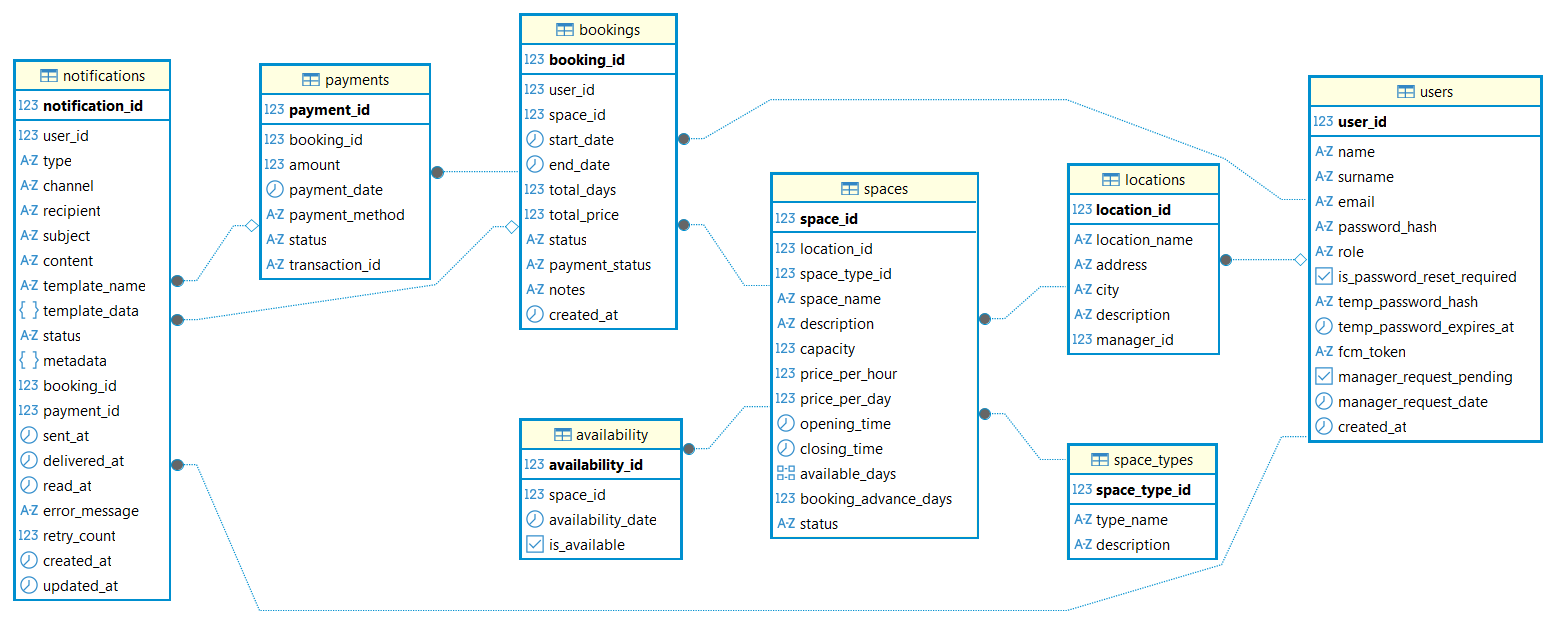
\includegraphics[width=\textwidth]{sections/ER_schema.png}
\caption{Diagramma ER del Sistema CoWorkSpace}
\label{fig:er_diagram}
\end{figure}

\subsection{Relazioni Principali}
\begin{itemize}
    \item \textbf{Users → Locations}: Un manager può gestire più sedi (1:N)
    \item \textbf{Locations → Spaces}: Una sede contiene più spazi (1:N)
    \item \textbf{Space Types → Spaces}: Un tipo può essere utilizzato da più spazi (1:N)
    \item \textbf{Spaces → Availability}: Ogni spazio ha disponibilità per più giorni (1:N)
    \item \textbf{Users → Bookings}: Un utente può fare più prenotazioni (1:N)
    \item \textbf{Spaces → Bookings}: Uno spazio può essere prenotato più volte (1:N)
    \item \textbf{Bookings → Payments}: Ogni prenotazione ha un unico pagamento (1:1)
    \item \textbf{Users → Notifications}: Un utente riceve più notifiche (1:N)
\end{itemize}

\subsection{Implementazione nel Progetto}

\subsubsection{Modelli JavaScript Implementati}
Il sistema CoWorkSpace implementa i seguenti modelli per gestire le operazioni database:

\begin{table}[H]
\centering
\begin{tabular}{@{}ll@{}}
\toprule
\textbf{Modello} & \textbf{File di Implementazione} \\
\midrule
User & \texttt{src/backend/models/User.js} \\
Location & \texttt{src/backend/models/Location.js} \\
Space & \texttt{src/backend/models/Space.js} \\
SpaceType & \texttt{src/backend/models/SpaceType.js} \\
Booking & \texttt{src/backend/models/Booking.js} \\
Payment & \texttt{src/backend/models/Payment.js} \\
Notification & \texttt{src/backend/models/Notification.js} \\
Availability & \texttt{src/backend/models/Availability.js} \\
\bottomrule
\end{tabular}
\caption{Modelli JavaScript del Sistema}
\end{table}

\subsubsection{Servizi di Business Logic}
Il sistema utilizza i seguenti servizi per implementare la logica di business:

\begin{table}[H]
\centering
\begin{tabular}{@{}lp{8cm}@{}}
\toprule
\textbf{Servizio} & \textbf{Responsabilità} \\
\midrule
AuthService & Autenticazione, autorizzazione, gestione ruoli \\
BookingService & Creazione prenotazioni, controllo disponibilità, calcolo prezzi \\
SpaceService & Gestione spazi, ricerca con filtri, validazioni \\
LocationService & Gestione sedi, assegnazione manager \\
NotificationService & Invio notifiche email e push \\
PaymentService & Gestione pagamenti, integrazione gateway \\
\bottomrule
\end{tabular}
\caption{Servizi di Business Logic}
\end{table}

\subsubsection{Validazioni e Constraints Implementati}
Il sistema implementa le seguenti validazioni a livello database e applicazione:

\begin{lstlisting}[caption=Constraint Database Implementati]
-- Validazioni email formato
CHECK (email ~* '^[A-Za-z0-9._%+-]+@[A-Za-z0-9.-]+\.[A-Za-z]{2,}$')

-- Validazioni date prenotazioni
CONSTRAINT booking_date_order CHECK (start_date <= end_date)
CONSTRAINT booking_future_date CHECK (start_date >= CURRENT_DATE)

-- Validazioni stati
CHECK (status IN ('active', 'maintenance', 'inactive'))
CHECK (type IN ('email', 'push', 'sms'))
\end{lstlisting}

\subsubsection{Sistema di Autorizzazioni}
Il sistema implementa un sistema di autorizzazioni a 3 livelli:

\begin{table}[H]
\centering
\begin{tabular}{@{}lp{10cm}@{}}
\toprule
\textbf{Ruolo} & \textbf{Permessi} \\
\midrule
\textbf{User} & Visualizzare spazi, creare prenotazioni, gestire proprio profilo \\
\textbf{Manager} & Tutti i permessi User + gestire location assegnate, spazi delle proprie location, visualizzare prenotazioni delle proprie location \\
\textbf{Admin} & Tutti i permessi + gestire utenti, promuovere manager, accesso completo al sistema \\
\bottomrule
\end{tabular}
\caption{Matrice dei Permessi per Ruolo}
\end{table}

\subsubsection{Configurazione Database}
Il sistema utilizza PostgreSQL con le seguenti configurazioni:

\begin{itemize}
    \item \textbf{Pool di connessioni}: Gestito tramite \texttt{pg} con retry automatico
    \item \textbf{Transazioni}: Supporto completo per operazioni atomiche
    \item \textbf{Prepared statements}: Utilizzo di query parametrizzate per sicurezza
    \item \textbf{Error handling}: Gestione specifica degli errori PostgreSQL
    \item \textbf{Logging}: Monitoraggio query lente e statistiche pool
\end{itemize}
\section{Operazioni CRUD}

Questa sezione descrive le operazioni di Create, Read, Update e Delete (CRUD) implementate nel sistema CoWorkSpace, con esempi pratici tratti direttamente dal codice del progetto.

\subsection{Gestione Utenti}

\subsubsection{Creazione Utente (CREATE)}
\begin{lstlisting}[caption=Registrazione Nuovo Utente (User.js)]
-- Query di inserimento utente dal modello User.js
INSERT INTO users (name, surname, email, password_hash, role, manager_request_pending, manager_request_date)
VALUES ($1, $2, $3, $4, $5, $6, $7)
RETURNING user_id, name, surname, email, role, created_at;
\end{lstlisting}

\subsubsection{Lettura Utenti (READ)}
\begin{lstlisting}[caption=Query per Login Utente]
-- Query di autenticazione dal modello User.js
SELECT * FROM users WHERE email = $1;
\end{lstlisting}

\begin{lstlisting}[caption=Ricerca Utenti con Paginazione]
-- Query implementata in UserService per admin
SELECT 
    user_id, name, surname, email, role, 
    manager_request_pending, created_at
FROM users 
WHERE 
    ($1 IS NULL OR role = $1)
    AND ($2 IS NULL OR LOWER(name || ' ' || surname) LIKE LOWER('%' || $2 || '%'))
ORDER BY created_at DESC
LIMIT $3 OFFSET $4;
\end{lstlisting}

\subsubsection{Aggiornamento Utente (UPDATE)}
\begin{lstlisting}[caption=Aggiornamento Profilo Utente Dinamico]
-- Query dinamica dal modello User.js per aggiornamento profilo
UPDATE users 
SET ${updateFields.join(', ')} 
WHERE user_id = $1 
RETURNING user_id, name, surname, email, role, created_at;

-- Esempio con campi: name = $2, surname = $3, fcm_token = $4
\end{lstlisting}

\begin{lstlisting}[caption=Aggiornamento Token FCM]
-- Query per notifiche push
UPDATE users 
SET fcm_token = $1 
WHERE user_id = $2 
RETURNING user_id, fcm_token;
\end{lstlisting}

\subsection{Gestione Spazi}

\subsubsection{Creazione Spazio (CREATE)}
\begin{lstlisting}[caption=Creazione Spazio dal Modello Space.js]
-- Query di inserimento spazio
INSERT INTO spaces (
    location_id, space_type_id, space_name, description, 
    capacity, price_per_hour, price_per_day, opening_time, closing_time
)
VALUES ($1, $2, $3, $4, $5, $6, $7, $8, $9)
RETURNING *;
\end{lstlisting}

\newpage

\subsubsection{Ricerca Spazi (READ)}
\begin{lstlisting}[caption=Query Completa Spazi con JOIN]
-- Query dal modello Space.js con tutti i dettagli
SELECT 
    s.*,
    l.location_name,
    l.address as location_address,
    l.city as location_city,
    st.type_name,
    st.description as space_type_description
FROM spaces s
INNER JOIN locations l ON s.location_id = l.location_id
INNER JOIN space_types st ON s.space_type_id = st.space_type_id
WHERE s.space_id = $1;
\end{lstlisting}

\begin{lstlisting}[caption=Ricerca Spazi Disponibili con Filtri]
-- Query per ricerca spazi con controllo disponibilità
SELECT DISTINCT s.*,
    l.location_name, l.city, l.address,
    st.type_name
FROM spaces s
INNER JOIN locations l ON s.location_id = l.location_id
INNER JOIN space_types st ON s.space_type_id = st.space_type_id
WHERE s.status = 'active'
    AND ($1 IS NULL OR LOWER(l.city) LIKE LOWER('%' || $1 || '%'))
    AND ($2 IS NULL OR s.capacity >= $2)
    AND ($3 IS NULL OR s.space_type_id = $3)
    AND NOT EXISTS (
        SELECT 1 FROM bookings b
        WHERE b.space_id = s.space_id
        AND b.status IN ('confirmed', 'pending')
        AND (b.start_date <= $4 AND b.end_date >= $5)
    )
ORDER BY s.price_per_day ASC;
\end{lstlisting}

\subsubsection{Aggiornamento Spazio (UPDATE)}
\begin{lstlisting}[caption=Aggiornamento Dinamico Spazio]
-- Query dinamica per aggiornamento spazi
UPDATE spaces 
SET ${fieldsToUpdate.join(', ')} 
WHERE space_id = $1
RETURNING *;

-- I campi vengono costruiti dinamicamente nel codice
\end{lstlisting}

\newpage

\subsection{Gestione Prenotazioni}

\subsubsection{Creazione Prenotazione (CREATE)}
\begin{lstlisting}[caption=Inserimento Prenotazione dal Modello Booking.js]
-- Query di inserimento prenotazione
INSERT INTO bookings (
    user_id, space_id, start_date, end_date,
    total_price, status, payment_status, notes
) VALUES ($1, $2, $3, $4, $5, $6, $7, $8)
RETURNING *;
\end{lstlisting}

\subsubsection{Ricerca Prenotazioni (READ)}
\begin{lstlisting}[caption=Query Prenotazione con Dettagli Completi]
-- Query dal modello Booking.js per ottenere tutti i dettagli
SELECT 
    b.*,
    u.name as user_name,
    u.surname as user_surname,
    u.email as user_email,
    s.space_name,
    s.capacity as space_capacity,
    s.price_per_hour,
    s.price_per_day,
    l.location_name,
    l.address as location_address,
    l.city as location_city
FROM bookings b
JOIN users u ON b.user_id = u.user_id
JOIN spaces s ON b.space_id = s.space_id
JOIN locations l ON s.location_id = l.location_id
WHERE b.booking_id = $1;
\end{lstlisting}

\subsubsection{Controllo Disponibilità}
\begin{lstlisting}[caption=Verifica Conflitti Prenotazioni]
-- Query per verificare sovrapposizioni dal BookingService
SELECT COUNT(*) as conflicts
FROM bookings
WHERE space_id = $1
    AND status IN ('confirmed', 'pending')
    AND (
        (start_date <= $2 AND end_date >= $2) OR
        (start_date <= $3 AND end_date >= $3) OR
        (start_date >= $2 AND end_date <= $3)
    );
\end{lstlisting}

\newpage

\subsubsection{Aggiornamento Prenotazione (UPDATE)}
\begin{lstlisting}[caption=Aggiornamento Stato Prenotazione]
-- Query dinamica dal modello Booking.js
UPDATE bookings 
SET ${fieldsToUpdate.join(', ')} 
WHERE booking_id = $1
RETURNING *;

-- Esempio per conferma: status = 'confirmed', payment_status = 'completed'
\end{lstlisting}

\subsection{Sistema di Notifiche}

\subsubsection{Creazione Notifica (CREATE)}
\begin{lstlisting}[caption=Inserimento Notifica dal Modello Notification.js]
-- Query di inserimento notifica
INSERT INTO notifications (
    user_id, type, channel, recipient, subject, content,
    template_name, template_data, booking_id, payment_id, status
) VALUES ($1, $2, $3, $4, $5, $6, $7, $8, $9, $10, $11)
RETURNING *;
\end{lstlisting}

\subsubsection{Aggiornamento Stato Notifica (UPDATE)}
\begin{lstlisting}[caption=Aggiornamento Stato Notifica]
-- Query per aggiornare stato notifica con timestamp
UPDATE notifications 
SET status = $1, metadata = $2, error_message = $3, sent_at = CURRENT_TIMESTAMP
WHERE notification_id = $4 
RETURNING *;
\end{lstlisting}

\newpage

\subsection{Gestione Locations e Space Types}

\subsubsection{Location CRUD}
\begin{lstlisting}[caption=Query Location dal Modello Location.js]
-- Inserimento location
INSERT INTO locations (location_name, address, city, description, manager_id)
VALUES ($1, $2, $3, $4, $5)
RETURNING *;

-- Ricerca locations con informazioni manager
SELECT 
    l.*,
    u.name as manager_name,
    u.surname as manager_surname,
    u.email as manager_email
FROM locations l
LEFT JOIN users u ON l.manager_id = u.user_id
WHERE ($1 IS NULL OR LOWER(l.city) LIKE LOWER('%' || $1 || '%'))
ORDER BY l.location_name;
\end{lstlisting}

\subsubsection{Space Types CRUD}
\begin{lstlisting}[caption=Query Space Types]
-- Ricerca tutti i tipi di spazio
SELECT * FROM space_types ORDER BY type_name;

-- Aggiornamento dinamico space type
UPDATE space_types 
SET ${updateFields.join(', ')} 
WHERE space_type_id = $1 
RETURNING *;
\end{lstlisting}
\newpage

\section{Esempi Specifici dal Progetto}

Questa sezione presenta esempi concreti di implementazione tratti direttamente dal codice del progetto CoWorkSpace, mostrando come le operazioni del database vengono utilizzate nelle funzionalità reali del sistema.

\subsection{Caso d'Uso: Sistema di Autenticazione}

Il sistema implementa un meccanismo completo di autenticazione con gestione ruoli.

\begin{lstlisting}[caption=Registrazione Utente con Validazioni (AuthService.js)]
// Logica di business per registrazione utente
const existingUser = await User.findByEmail(email);
if (existingUser) {
    throw AppError.badRequest('Email già registrata');
}

// Hash della password
const saltRounds = 12;
const password_hash = await bcrypt.hash(password, saltRounds);

// Creazione utente con ruolo di default
const userData = {
    name, surname, email, password_hash,
    role: 'user',  // Ruolo di default
    manager_request_pending: false
};

const user = await User.create(userData);
return user;
\end{lstlisting}

\begin{lstlisting}[caption=Query SQL di Registrazione Utente]
-- Query effettiva dal modello User.js
INSERT INTO users (name, surname, email, password_hash, role, manager_request_pending, manager_request_date)
VALUES ($1, $2, $3, $4, $5, $6, $7)
RETURNING user_id, name, surname, email, role, created_at;
\end{lstlisting}

\newpage

\subsection{Caso d'Uso: Creazione Spazio con Validazioni Business}

Il seguente esempio mostra la logica completa di creazione di uno spazio implementata nel sistema.

\begin{lstlisting}[caption=Creazione Spazio con Autorizzazioni (SpaceService.js)]
// Validazione autorizzazioni dal SpaceService
if (!['admin', 'manager'].includes(currentUser.role)) {
    throw AppError.forbidden('Non hai i permessi per creare uno spazio');
}

// Verifica esistenza location
const location = await Location.findById(spaceData.location_id);
if (!location) {
    throw AppError.badRequest('Location non trovata');
}

// I manager possono creare spazi solo nelle loro location
if (currentUser.role === 'manager' && 
    location.manager_id !== currentUser.user_id) {
    throw AppError.forbidden('Puoi creare spazi solo nelle tue location');
}

// Calcolo automatico prezzo giornaliero se non fornito
if (!spaceData.price_per_day && spaceData.price_per_hour) {
    spaceData.price_per_day = Space.calculateDailyPrice(
        spaceData.price_per_hour, 
        spaceData.opening_time, 
        spaceData.closing_time
    );
}

return await Space.create(spaceData);
\end{lstlisting}

\begin{lstlisting}[caption=Query SQL di Creazione Spazio]
-- Query effettiva dal modello Space.js
INSERT INTO spaces (
    location_id, space_type_id, space_name, description, 
    capacity, price_per_hour, price_per_day, opening_time, closing_time
)
VALUES ($1, $2, $3, $4, $5, $6, $7, $8, $9)
RETURNING *;
\end{lstlisting}

\newpage

\subsection{Caso d'Uso: Processo di Prenotazione}

Il sistema implementa un processo di prenotazione che include validazioni e controllo disponibilità.

\begin{lstlisting}[caption=Creazione Prenotazione con Validazioni (BookingService.js)]
// Validazione disponibilità spazio
const space = await Space.findById(spaceData.space_id);
if (!space) {
    throw AppError.badRequest('Spazio non trovato');
}

// Controllo conflitti prenotazioni esistenti
const conflicts = await this.checkBookingConflicts(
    spaceData.space_id, 
    spaceData.start_date, 
    spaceData.end_date
);

if (conflicts > 0) {
    throw AppError.conflict('Spazio già prenotato nelle date selezionate');
}

// Calcolo prezzo totale
const totalPrice = await this.calculateBookingPrice(
    space,
    spaceData.start_date,
    spaceData.end_date
);

// Creazione prenotazione
const bookingData = {
    user_id: currentUser.user_id,
    space_id: spaceData.space_id,
    start_date: spaceData.start_date,
    end_date: spaceData.end_date,
    total_price: totalPrice,
    status: 'pending',
    payment_status: 'pending',
    notes: spaceData.notes
};

const booking = await Booking.create(bookingData);
return booking;
\end{lstlisting}

\begin{lstlisting}[caption=Query Controllo Conflitti Prenotazioni]
-- Query dal BookingService per verificare sovrapposizioni
SELECT COUNT(*) as conflicts
FROM bookings
WHERE space_id = $1
    AND status IN ('confirmed', 'pending')
    AND (
        (start_date <= $2 AND end_date >= $2) OR
        (start_date <= $3 AND end_date >= $3) OR
        (start_date >= $2 AND end_date <= $3)
    );
\end{lstlisting}

\subsection{Caso d'Uso: Sistema di Autorizzazioni}

Il sistema implementa controlli di autorizzazione granulari per ogni operazione.

\begin{lstlisting}[caption=Middleware di Autorizzazione (authMiddleware.js)]
// Controllo ruoli da authMiddleware.js
const requireRole = (roles) => {
    return (req, res, next) => {
        if (!req.user) {
            return next(AppError.unauthorized('Token richiesto'));
        }

        if (!roles.includes(req.user.role)) {
            return next(AppError.forbidden(
                `Accesso negato. Ruoli richiesti: ${roles.join(', ')}`
            ));
        }

        next();
    };
};

// Utilizzo nei controller
exports.createSpace = [
    requireRole(['admin', 'manager']),
    catchAsync(async (req, res) => {
        // Logica creazione spazio
    })
];
\end{lstlisting}

\subsection{Caso d'Uso: Gestione Manager per Location}

Il sistema permette ai manager di gestire solo le proprie location.

\begin{lstlisting}[caption=Validazione Ownership Manager (LocationService.js)]
// Controllo ownership location per manager
static async canManageLocation(location, currentUser) {
    if (currentUser.role === 'admin') {
        return true; // Admin può tutto
    }
    if (currentUser.role === 'manager') {
        return location.manager_id === currentUser.user_id;
    }
    return false; // User non può gestire location
}
// Utilizzo nel controller
const location = await Location.findById(locationId);
if (!location) {
    throw AppError.notFound('Location non trovata');
}

const canManage = await LocationService.canManageLocation(location, req.user);
if (!canManage) {
    throw AppError.forbidden('Non puoi gestire questa location');
}
\end{lstlisting}

\subsection{Caso d'Uso: Dashboard Analytics Semplici}

Il sistema fornisce statistiche base per manager e admin.

\begin{lstlisting}[caption=Statistiche Dashboard Manager (BookingService.js)]
// Query per dashboard manager
static async getBookingsDashboard(currentUser, filters = {}) {
    let baseQuery = `
        SELECT 
            COUNT(*) as total_bookings,
            SUM(CASE WHEN status = 'confirmed' THEN 1 ELSE 0 END) as confirmed_bookings,
            SUM(CASE WHEN status = 'pending' THEN 1 ELSE 0 END) as pending_bookings,
            SUM(total_price) as total_revenue
        FROM bookings b
        INNER JOIN spaces s ON b.space_id = s.space_id
        INNER JOIN locations l ON s.location_id = l.location_id
    `;

    const conditions = ['1=1'];
    const queryParams = [];

    // Filtro per manager: solo le sue location
    if (currentUser.role === 'manager') {
        conditions.push('l.manager_id = $' + (queryParams.length + 1));
        queryParams.push(currentUser.user_id);
    }

    const finalQuery = baseQuery + ' WHERE ' + conditions.join(' AND ');
    const result = await pool.query(finalQuery, queryParams);
    
    return result.rows[0];
}
\end{lstlisting}

\subsection{Caso d'Uso: Sistema di Notifiche Base}

Il sistema implementa notifiche semplici per eventi importanti.

\begin{lstlisting}[caption=Creazione Notifica Email (NotificationService.js)]
// Creazione notifica booking confermato
static async createBookingConfirmationNotification(booking) {
    const notificationData = {
        user_id: booking.user_id,
        type: 'email',
        channel: 'booking_confirmation',
        recipient: booking.user_email,
        subject: `Prenotazione Confermata - ${booking.space_name}`,
        content: `La tua prenotazione per ${booking.space_name} dal ${booking.start_date} al ${booking.end_date} è stata confermata.`,
        booking_id: booking.booking_id,
        status: 'pending'
    };
    return await Notification.create(notificationData);
}
\end{lstlisting}

\begin{lstlisting}[caption=Query Inserimento Notifica]
-- Query dal modello Notification.js
INSERT INTO notifications (
    user_id, type, channel, recipient, subject, content,
    template_name, template_data, booking_id, payment_id, status
) VALUES ($1, $2, $3, $4, $5, $6, $7, $8, $9, $10, $11)
RETURNING *;
\end{lstlisting}

\subsection{Caso d'Uso: Gestione Errori e Validazioni}

Il sistema implementa validazioni robuste e gestione errori centralizata.

\begin{lstlisting}[caption=Gestione Errori Database (Booking.js)]
// Gestione errori specifici PostgreSQL
try {
    const result = await pool.query(query, values);
    return new Booking(result.rows[0]);
} catch (error) {
    // Foreign key violation
    if (error.code === '23503') {
        if (error.constraint?.includes('user_id')) {
            throw AppError.badRequest('Utente non valido');
        }
        if (error.constraint?.includes('space_id')) {
            throw AppError.badRequest('Spazio non valido');
        }
    }
    
    // Check constraint violation
    if (error.code === '23514') {
        if (error.constraint?.includes('booking_date_order')) {
            throw AppError.badRequest('La data di inizio deve essere precedente a quella di fine');
        }
        if (error.constraint?.includes('booking_future_date')) {
            throw AppError.badRequest('La prenotazione deve essere per una data futura');
        }
    }
    
    throw AppError.internal('Errore durante la creazione della prenotazione', error);
}
\end{lstlisting}

\newpage

\subsection{Caso d'Uso: Aggiornamento Dinamico dei Campi}

Il sistema implementa aggiornamenti dinamici per evitare query ridondanti.

\begin{lstlisting}[caption=Update Dinamico Utente (User.js)]
// Costruzione dinamica query di aggiornamento
async updateProfile(updateData) {
    const allowedFields = ['name', 'surname', 'fcm_token'];
    const updateFields = [];
    const queryParams = [this.user_id];
    let queryIndex = 2;

    for (const [key, value] of Object.entries(updateData)) {
        if (allowedFields.includes(key) && value !== undefined && value !== '') {
            updateFields.push(`${key} = $${queryIndex++}`);
            queryParams.push(value);
        }
    }

    if (updateFields.length === 0) {
        throw AppError.badRequest('Nessun campo valido fornito per l\'aggiornamento');
    }

    const query = `UPDATE users SET ${updateFields.join(', ')} WHERE user_id = $1 RETURNING *`;
    const result = await pool.query(query, queryParams);
    
    return result.rows[0];
}
\end{lstlisting}

\end{document}